\section{Mediator}


Nesse padrão, um objeto chamado de Mediator age como intermediário 
entre um grupo de objetos, ficando responsável por qualquer 
interação entre eles. O Mediator conhece todos 
esses objetos, enquanto cada objeto conhece apenas o 
Mediator, o que os torna 
mais independentes, simplificando sua reutilização
 e concentrando as dependências entre eles 
em um só lugar. 

A estrutura do padrão é apresentada na figura \ref{mediator_struct}. 
Uma interface Mediator define as operações que um tipo de 
objeto Mediator deve possuir. ConcreteMediator representa 
uma classe que implementa essas operações. Um Colleague 
é um objeto conhecido pelo Mediator e cada ConcreteColleague 
pode ser tanto um objeto que possui operações refletidas 
em outros objetos quanto ser um dos objetos afetados 
indiretamente por outro Colleague.

\begin{figure}[htb]
	\caption{\label{mediator_struct}Estrutura do Mediator}
	\begin{center}
	    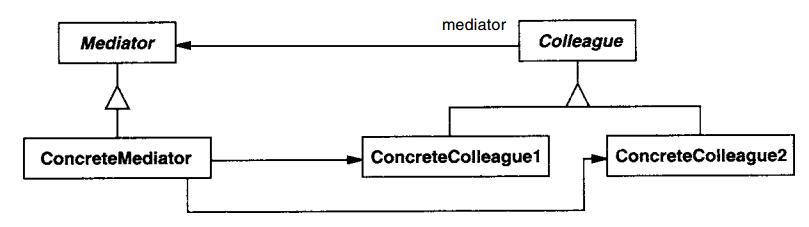
\includegraphics[scale=0.5]{5_padroes-contexto-funcional/5.3_comportamentais/5.3.05_mediator/diagram.png}
	\end{center}
\end{figure}



\subsection*{Exemplo Orientado a Objetos}

Como exemplo, é considerada uma janela de uma aplicação 
que apresenta diversos \textit{widgets}, entre eles uma caixa 
de entrada de texto e uma lista de seleção. Quando um item é 
selecionado na lista, o texto contido nele deve aparecer 
na caixa de entrada de texto. O Mediator é responsável 
por alterar a caixa de entrada de texto quando um item 
é selecionado na lista, enquanto a lista é responsável 
por informar ao Mediator quando um item for selecionado. 
A figura \ref{mediator_exemplo} apresenta o diagrama 
de classes para esse exemplo. O código \ref{oomediator} 
apresenta a implementação do padrão para esse exemplo.

\begin{figure}[htb]
	\caption{\label{mediator_exemplo}Exemplo de Mediator}
	\begin{center}
	    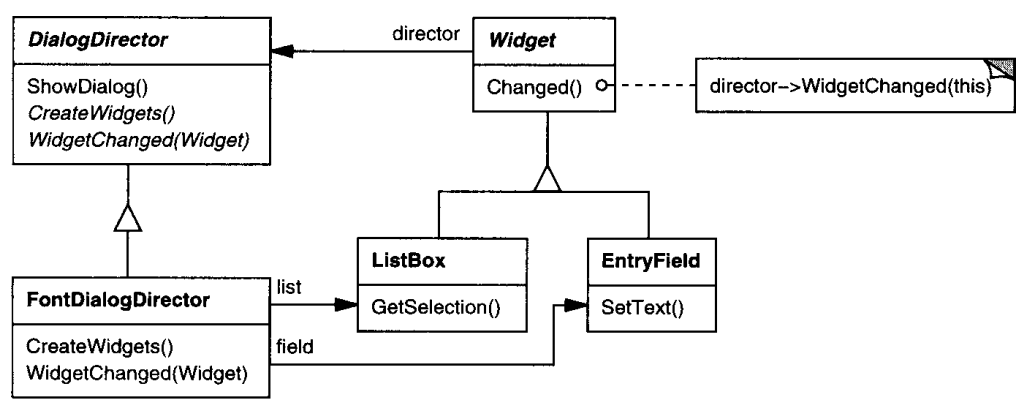
\includegraphics[scale=0.4]{5_padroes-contexto-funcional/5.3_comportamentais/5.3.05_mediator/exemplo_mediator.png}
	\end{center}
\end{figure}

\begin{lstlisting}[caption={Mediator Orientado a Objetos},label=oomediator]

trait DialogDirector {
    
    def ShowDialog() {
        // Operação que exibe o Dialog
    }

    def CreateWidgets() : Unit
    def WidgetChanged(widget : Widget) : Unit
}

class FontDialogDirector extends DialogDirector {
    
    val list : ListBox
    val field : EntryField
    
    def CreateWidgets() {
        this.list = new ListBox(this)
        this.field = new EntryField(this)
    }

    def WidgetChanged(widget : Widget) {
        this.field.SetText(
            this.list.GetSelection()
        )
    }

}

abstract class Widget(val director : DialogDirector){

    def Changed() : Unit = this.director.WidgetChanged(this)

}

class EntryField(director : DialogDirector) extends Widget(director) {
    var text : String

    def SetText(text : String) {
        this.text = text
    }
}

class ListBox(director : DialogDirector) extends Widget(director){
    var selection : String

    def GetSelection() : String = selection

    def SetSelection(selection : String) {
        this.selection = selection
        Changed()
    }
}
    
\end{lstlisting}

\subsection*{Contexto Funcional}

Como o objetivo do padrão é gerenciar as interdependências 
entre elementos diferentes sem que eles precisem se conhecer, 
o objeto ConcreteMediator pode ser equivalente a um módulo 
que define as funções que serão executadas nos Colleagues 
afetados quando algum Colleague alvo realizar uma operação. 
Para simplificar a descrição do exemplo funcional, será 
definido como "Colleague alvo" um Colleague que, no 
exemplo orientado a objetos, teria executado uma operação 
que avisa o Mediator e "Colleague afetado" como um 
Colleague que, após o Mediator ter sido avisado, foi 
modificado ou referenciado. É importante notar que qualquer 
Colleague pode agir tanto como alvo quanto como afetado, 
dependedo do contexto.

Como as funções devem ser puras, uma função de um Colleague 
alvo não pode modificar um Colleague afetado sem que o mesmo seja 
passado por parâmetro. Seguindo essa abordagem, os Colleagues 
tornariam-se dependentes uns dos outros novamente, o que não 
é desejado. Uma forma de resolver esse problema é trazendo 
para o Mediator a responsabilidade de chamar as operações 
dos Colleagues de forma que as funções do Mediator serão 
compostas por uma função que faz a modificação no Colleague alvo  
e de todas as funções necessárias para modificar os 
Colleagues afetados. Essas funções podem receber como parâmetro 
os valores necessários para modificar o Colleague alvo, 
mas para que a abordagem seja equivalente à orientda a 
objetos, elas não deveriam receber nenhum parâmetro 
exclusivo das funções que alteram os Colleagues afetados. 
Outra consequência do uso de funções puras, que também 
é uma consequência da imutabilidade, é que também será 
responsabilidade das funções do Mediator retornar todos 
os Colleagues alterados.

O código \ref{fpmediator} demonstra o exemplo visto 
anteriormente utilizando as ideias apresentadas. Um módulo 
FontDialogDirector possui a operação ChangeWidget, que 
trabalha com os tipos abstratos A, representando o tipo 
do Colleague alvo e B representando o tipo do Colleague 
afetado. Como a função ChangeWidget não define a forma 
como os Colleagues afetados são alterados, o tipo B pode 
ser tanto um único Colleague quanto uma tupla ou lista 
de Colleagues afetados. A função ChangeWidget também 
recebe uma função que recebe como parâmetros valores 
dos tipos A e B e retorna uma tupla contendo valores 
dos mesmos tipos. A implementação da função é apenas a chamada 
de f para os widgets dos tipos A e B recebidos como entrada.

A função f recebida como parâmetro é responsável por 
definir qual função do Colleague alvo será chamada e 
como isso modificará os Colleagues afetados. No exemplo, 
ela pode ser definida através da função ChangeSelectionFunction, 
que recebe como parâmetro o valor da seleção para o \textit{widget} 
de lista de seleção e retorna uma função que recebe como parâmetro 
um ListBox como Colleague alvo e um EntryField como 
Colleague afetado. O valor da seleção será armazenado 
em uma closure e será utilizado na chamada das funções 
SetSelection e SetText. Essa abordagem contribui 
para que novas funções para valores diferentes de 
seleção não precisem ser criadas e também para que 
uma mesma função que seleciona um valor possa ser 
reutilizada por mais de um \textit{widget} da aplicação.

\begin{lstlisting}[caption={Mediator Funcional},label=fpmediator]
    
	object FontDialogDirector {

		import EntryField._
		import ListBox._
	
		def ChangeWidget[A, B](
			changedWidget : A,
			affectedWidgets : B,
			f : (A, B) => (A, B)) 
		: (A, B) = f(changedWidget, affectedWidgets)
	
	
		def ChangeSelectionFunction(selection : String) = 
			(listBox : ListBox, entryField : EntryField) => 
				(SetSelection(listBox, selection), 
				 SetText(entryField, selection))
	
	}
	
	object EntryField {
	
		case class EntryField(val text : String)
	
		def SetText(entryField : EntryField, text : String) = 
			entryField.copy(text)
		
		def GetText(entryField : EntryField) = 
			entryField.text
	}
	
	object ListBox {
	
		case class ListBox(val selection : String)
		
		def SetSelection(listBox : ListBox, selection : String) = 
			listBox.copy(selection=selection)
		
		def GetSelection(listBox : ListBox) = 
			listBox.selection
	}
	
    
\end{lstlisting}

\subsection*{Vantagens e Desvantagens}

Uma vantagem observável da abordagem funcional é 
que os colleagues não precisam conhecer o Mediator. 
Dessa forma, os \textit{widgets} poderiam ser 
reutilizados em outros trechos da aplicação onde 
eles não precisam depender ou ser dependentes 
de outros elementos. 

Uma desvantagem é o gerenciamento dos \textit{widgets}, 
já que é sempre necessário desestruturar a tupla retornada 
pela função ChangeWidget para recuperar os novos 
valores. Essa operação pode tornar-se ainda mais 
difícil se a quantidade de Colleagues afetados 
aumentar ou se eles estiverem organizados em uma estrutura 
mais complexa. Outra desvantagem é que as operações 
precisam passar explicitamente pelo Mediator para 
serem executadas, tornando uma refatoração 
onde o Mediator não é mais necessário mais custosa.